\section{Sample output of first stage model}

This was only the first of the many hurdles I faced. This is not completely a surprise,
due to the complex nature of internal combustion
models, but the first stage model was quite fragile. It is highly sensitive to
input parameters and initial guesses, and the existence of a rocket with a given
burn profile is not
guaranteed even with significant relaxations of the conservation laws. However, I was
able to extract aggregate geometric information for a constant burn rocket, which I present
here and use in the rest of the project. The rocket in question burns at a constant thrust
of $150\rm{kN}$ for 4 seconds. The area and circumference evolution of the cross section of the rocket
are shown in Figure~\ref{fig:profiles}.

\begin{figure}
    \begin{subfigure}{0.48\textwidth}
        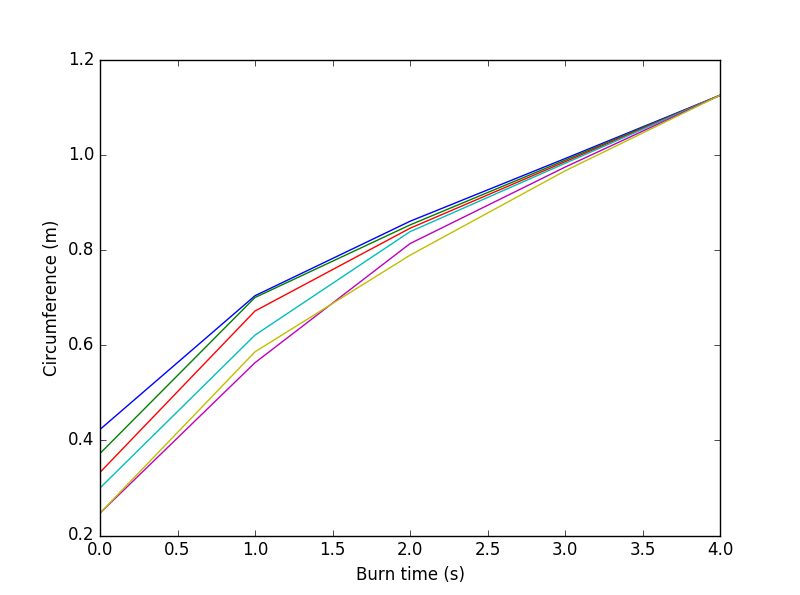
\includegraphics[width = 0.9\linewidth]{figures/cprofile.png}
        \caption{Cross-sectional circumference evolution}
        \label{fig:csec}
    \end{subfigure}
    \begin{subfigure}{0.48\textwidth}
        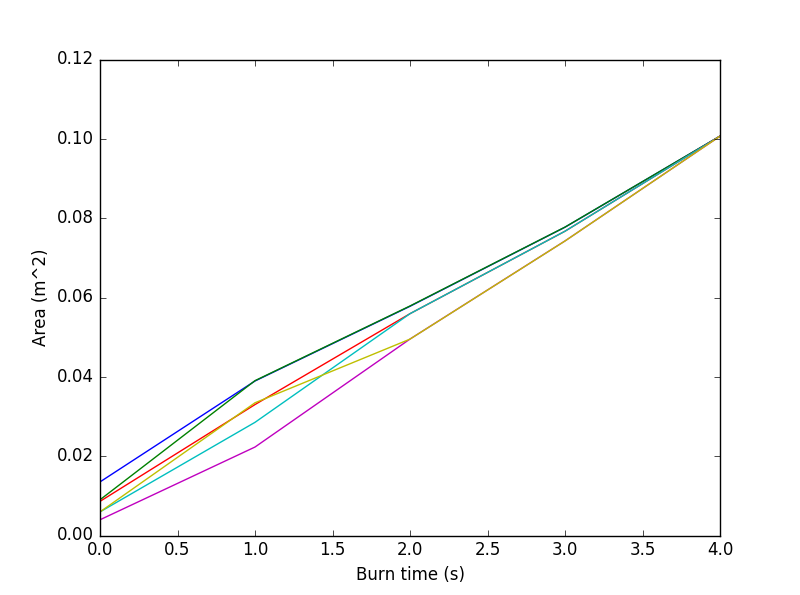
\includegraphics[width = 0.9\linewidth]{figures/aprofile.png}
        \caption{Cross-sectional area evolution}
        \label{fig:asec}
    \end{subfigure}
    \caption{Evolution of the cross-section of the rocket at 6 axial locations.}
    \label{fig:profiles}
\end{figure}

For the rest of the report, we will be focusing on mapping the cross-sectional
area and circumference evolution of the blue curve onto polynomials.
